\section{Stratégie}

\begin{itemize}
  \item \emph{Data \& Modeling: What data model and representation model should you use in your Hive database? Why?  What issues will you have to deal with if you have to manage the same data  type for 10 million sites?}
\end{itemize}

\par Pour mener à bien le projet, notre équipe propose une stratégie en trois étapes. Toutes les mesures seront accumulées dans une table externe all\_records. C’est une table en ligne et les fichiers y sont stockés au format TEXTFILE (cela revient à concaténer tous nos csv). Cette table représente un niveau immuable des données, les lignes n’y sont ni modifiées ni supprimées. On s’appuie sur elles pour effectuer les requêtes de remplissage des tables de travail : work\_table<description>. Cette fois, la table est interne et la donnée y est compressée. Le modèle de données et les requêtes de remplissage dépendent alors de la portée de l’étude (ceux que nous avons exploités seront décrits dans cette partie). Enfin, le résultat des différentes agrégations est stocké dans des vues HIVE afin d’y simplifier l’accès.

\section{Modélisation}

\subsection{Point de départ: les tables Enernoc}

\begin{figure}[h!]
\centering
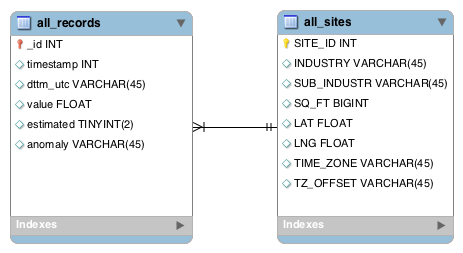
\includegraphics[scale=0.5]{./image/ER.png}
\caption{Entité-Relation relative aux tables de départ fournies pas Enernoc}
\end{figure}

\begin{block}{Note}
Lien entre \sqlcmd{all\_site} et \sqlcmd{all\_records}. Dès les premières injections de données et créations de table il semble évidant que le lien entre ces deux tables nécessite une jointure. Celle-ci se réalise sur les champs : \sqlcmd{all\_sites.SITE\_ID} et \sqlcmd{all\_records}. Comme expliqué en III.1 dans la description des fichiers, les mesures portent en nom de fichier l’id du site mais il ne se retrouve pas dans les colonnes. Nous effectuons donc la jointure sur la méta donnée \sqlcmd{INPUT\_\_FILE\_\_NAME} qui retourne l'adresse complète de la ressource.
(ex: \textcolor{blue}{hdfs://ns3099426....eu:8020/apps/hive/warehouse/project.db/enernoc/474.csv} ) Notre première UDF consistera alors à parser ce chemin pour obtenir l’id, ici \textbf{474}. Cette infomation est accessible pour chaque ligne de la table.
\end{block}

\begin{figure}[h!]
\centering
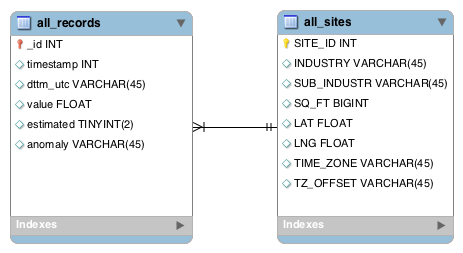
\includegraphics[scale=0.5]{./image/ER.png}
\begin{lstlisting}[language=java]
public Text evaluate(Text input){
  	if (input == null) return new Text("");
		final String path = input.toString();
		final int index = path.lastIndexOf("/");
		final int offset = path.lastIndexOf(".");
		return new Text(path.substring(index + 1, offset));
	}
\end{lstlisting}
\end{figure}

\subsection{Difficultés rencontrées liées à la modélisation: La table colonne}
\subsection{Les solutions privilégiées}
